\documentclass[12pt]{scrartcl}
\usepackage[latin1]{inputenc}
\usepackage{palatino}
\usepackage[bahasa]{babel}
\usepackage{microtype}
\usepackage{graphicx}
\usepackage{hyphenat}
\usepackage[paperwidth=74.00mm, paperheight=105.00mm, left=1cm, right=1cm, top=1cm, bottom=1cm, showframe]{geometry}
\author{Yohanes Suyanto}
\hyphenation{A-len-con a-nak a-nak-nya te-man te-man-nya}
\begin{document}
\sloppy
\thispagestyle{empty}
\begin{center}
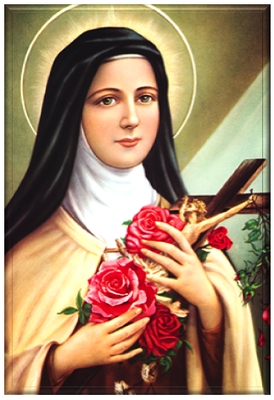
\includegraphics[scale=2.5]{st-theresia-kanak2.png}

St. Theresia dari Kanak-kanak Yesus
\end{center}

\newpage
\scriptsize
\subsection*{Santa Theresia dari Kanak-kanak Yesus}
\subsubsection*{Perawan dan Pelindung Karya Misi}

Maria Francoise Therese Martin lahir di Alencon, Prancis pada tanggal 2 Januari 1873. Theresia adalah puteri bungsu dari keluarga saleh Louis Martin dan Azelie Guerin. Ayahnya seorang pembuat arloji di kota Alencon. Sepeninggal isterinya, ia bersama a\-nak-a\-nak\-nya pindah ke Lisieux. Kematian ibunya menimbulkan shock besar pada Theresia sebagai puteri bungsu. Terpaksa kakaknya, Pauline, menggantikan kedudukan ibunya untuk merawat dan memperhatikan perkembangannya.

Theresia sangat dikasihi ayahnya. Ia diberi macam-macam julukan: 'Theresia Kecil', 'Bungsu Kecil' dan 'Ratu Kecil'. Pada tahun 1881 sampai 1885, ia belajar di sekolah Suster-suster Benediktin. Ia sangat perasa dan cepat menangis sehingga teman\hyp{}temannya tidak akrab dengannya. Ia semakin menjadi perasa sewaktu kakaknya Pauline masuk biara Karmelit di Lisieux pada bulan Oktober 1882. Theresia jatuh sakit karena keberangkatan Pauline itu. Theresia disembuhkan secara ajaib. Sementra kakak-kakaknya berlutut disamping tempat tidurnya untuk berdoa bagi kesembuhannya, patung Bunda Maria yang berada di depannya tiba-tiba tersenyum padanya. Penyakit itu hilang seketika meskipun sifat perasa masih tetap ada. Sifat itu baru mulai hilang karena nasehat ayahnya ketika mereka menghadiri upacara malam Natal tahun 1886. Semenjak itu, ia mulai semakin sadar akan keburukan dari sifatnya yang manja dan lekas tersinggung itu. Ia sadar bahwa ia sudah mulai remaja dan lebih dari itu bahwa sifat kekanak-kanakan itu tidak cocok bagi seorang wanita yang bercita-cita menjadi suster. Saat kesadarannya ini -- kemudian dalam autobiografinya -- disebutnya sebagai saat ber-rahmat yang mengawali kehidupannya yang baru. Katanya dalam buku itu: "Yesuslah yang merubah diriku."

Semenjak itu ia mulai sadar bahwa dirinya dipenuhi karunia Roh Kudus. Ia sadar pula bahwa dia harus mengabdikan seluruh-hidupnya kepada Tuhan. Kerinduannya untuk bersatu dengan Kanak-kanak Yesus sangatlah besar, dan karena itu di kemudian hari setelah ia digelari 'kudus', ia dinamai 'Theresia dari Kanak-kanak Yesus' dan Theresia dari Lisieux'. Kepada Yesus ia berjanji tidak akan pernah segan melakukan apa saja yang dikehendaki Tuhan dari padanya.

Kerinduannya itu terungkap dalam salah satu doanya berikut ini: "Yesus, tentu Engkau senang mempunyai mainan. Biarlah saya menjadi mainanMu! Anggap saja saya ini mainanMu. Bila akan Kauangkat, betapa senang hatiku. Jika hendak Kausepak kian kemari, silakan!' Dan kalau hendak Kautinggalkan di pojok kamar lantaran bosan, boleh saja. Saya akan menunggu dengan sabar dan setia. Tetapi kalau hendak Kautusuk bolaMu. . .O, Yesus, tentu itu sakit sekali, namun terjadilah kehendakMu!" Inilah doa Theresia Martin kepada Kanak-kanak Yesus yang sangat dirindukannya tetapi belum bisa disambutnya karena umurnya baru 7 tahun.

Orangtua Theresia baik sekali terhadapnya bersama saudara-saudaranya yang lain. Mereka semua - ada lima orang - menjadi suster. Betapa bahagia hati Theresia, ketika pada umur 12 tahun boleh menyambut Tubuh Yesus untuk pertama kalinya. Di hadapan sebuah salib, ia berjanji: "Yesus di kayu salib yang haus, saya akan 'memberikan air kepadaMu. Saya bersedia menderita sedapat mungkin, agar banyak orang berdosa bertobat." Pendosa pertama yang bertobat berkat doa Theresia ialah seorang penjahat kakap yang dijatuhi hukuman mati tanpa menyesal, namun akhirnya ia bertobat juga di hadapan sebuah salib sesaat sebelum menjalani hukuman.

Kerinduan Theresia yang begitu besar pada Yesus mendesak dia untuk menjalani kehidupan khusus sebagai seorang biarawati, mengikuti teladan 4 orang saudaranya yang sudah lebih dahulu menjadi suster. Tetapi ia belum bisa diterima karena umurnya baru 14 tahun. Ia tidak putus asa. Ia. berziarah ke Roma bersama orangtuanya. Dalam audiensi umum dengan Bapa Suci, ia dengan berani meminta izin khusus dari Bapa Suci untuk menjadi suster. Permintaannya itu dikabulkan dan dia boleh masuk biara pada umur 15 tahun. Ia diterima dalam biara Suster-suster Karmelit di Lisieux, Prancis. Kedua kakaknya sudah lebih dahulu di biara itu. Sembilan tahun lamanya, ia hidup sebagai suster biasa. Sebagaimana suster muda lainnya, ia melaksanakan tugas dan doa harian, harus mengatasi perasaan tersinggung, marah, rasa iri hati dan memerangi kebosanan serta bermacam ragam godaan lahir maupun batin. Untuk mencapai kesempurnaan hidup, ia memilih 'jalan sederhana' berdasarkan ajaran Kitab Suci: hidup selaku seorang anak kecil, penuh cinta dan iman kepercayaan akan Allah dan penyerahan diri yang total dengan perasaan gembira. Demi cita-cita itu, ia melakukan hal-hal kecil dan kewajiban-kewajiban sehari-hari dengan penuh tanggungjawab karena cinta kasihnya yang besar kepada Allah Bapa di surga.

Ia sedih sekali melihat banyak orang menyakiti hati Yesus dengan berbuat dosa dan tidak mau bertobat. Untuk mempertobatkan orangorang berdosa itu, ia mempersembahkan dirinya sebagai korban penyilih dosa-dosa. Ia rajin berdoa dan melakukan tapa bagi semua orang berdosa. Ia juga berdoa bagi para misionaris dan kemajuan Kerajaan Allah di seluruh dunia.

Theresia akhirnya menderita sakit paru-paru yang parah. Selama dua tahun lamanya ia menanggung beban penderitaan itu dengan gembira. Penyakit ini kemudian merengut nyawanya pada tanggal 30 September 1897 di biara Lisieux. Sebelum menghembuskan nafasnya, ia berjanji untuk menurunkan hujan mawar ke dunia. Janji ini benar terpenuhi karena banyak karunia Allah diberikan kepada semua orang yang berdoa dengan perantaraannya.

Theresia meninggal dunia dalam usia yang sangat muda, 24 tahun. Ia mewariskan catatan riwayat pribadinya yang ditulis atas permintaan ibu biara: "Kisah suatu Jiwa." Di dalamnya ia menunjukkan bahwa kesucian hidup dapat dicapai oleh siapa saja, betapa pun rendah, hina dan biasa orang itu. Caranya ialah melaksanakan pekerjaan-pekerjaan kecil dan tugas sehari-hari dengan penuh cintakasih yang murni kepada Tuhan.

Theresia adalah seorang Suster Karmelit yang terkenal di Prancis pada abad 20. Pada tahun 1925, ia digelari sebagai 'santa' oleh Paus Pius XI (1922-1939) dan diangkat sebagai 'Pelindung Karya Misi Gereja'. Kemudian oleh Paus Pius XII (1939-1958), Theresia diangkat sebagai 'Pelindung Prancis'.

\end{document}